\documentclass[aspectratio=169, 10pt]{beamer}
\usetheme{metropolis}
% \usefonttheme{professionalfonts}

\usepackage[english]{babel}
\usepackage[style=authortitle,backend=biber]{biblatex}
\usepackage[utf8]{inputenc}
\usepackage{algorithmic}
\usepackage{amsfonts}
\usepackage{amsmath}
\usepackage{amssymb}
\usepackage{array}
\usepackage{booktabs}
\usepackage{caption}
\usepackage{colortbl}
\usepackage{csquotes}
\usepackage{graphicx}
\usepackage{heuristica}
\usepackage{hyperref}
\usepackage{mathptmx}
\usepackage{multirow}
\usepackage{pgfplots}
\usepackage{siunitx}
\usepackage{subcaption}
\usepackage{svg}
\usepackage{tabularx}
\usepackage{textcomp}
\usepackage{xcolor}
\usepackage{bm}

\addbibresource{references.bib}

\usetikzlibrary{calc}

% \pgfplotsset{compat=1.17}
\usepgfplotslibrary{statistics}

\definecolor{uniblue}{HTML}{00467f}
\definecolor{uniblueDark}{HTML}{002052}
\definecolor{uniblueLight}{HTML}{4671af}
\definecolor{blueGrey}{HTML}{cfd8dc}
\definecolor{red800Dark}{HTML}{8e0000}
\definecolor{green800Dark}{HTML}{005005}

\setbeamercolor{background canvas}{bg=white}
% \setbeamertemplate{frame footer}{\insertshortauthor}
\setbeamerfont{page number in head/foot}{size=\tiny}
% \setbeamercolor{footline}{fg=white, bg=uniblue}
\setbeamercolor{footline}{fg=uniblue}
\setbeamercolor{title}{fg=uniblueDark, bg=white}
\setbeamercolor{frametitle}{fg=white, bg=uniblue}
\setbeamercolor{progress bar}{fg=uniblueLight, bg=white}
\setbeamercolor{block title}{use=structure,fg=white,bg=uniblue}
\setbeamercolor{block body}{use=structure,fg=black,bg=blueGrey}
\setbeamercolor{block title alerted}{fg=white,bg=red800Dark}
\setbeamercolor*{block title example}{fg=white, bg=green800Dark}
\setbeamercolor{alerted text}{fg=red800Dark}
\setbeamercolor{footnote}{fg=black}
\setbeamertemplate{frametitle continuation}[from second]
\setbeamercolor*{bibliography entry title}{fg=black}
\setbeamercolor*{bibliography entry author}{fg=black}
\setbeamercolor*{bibliography entry location}{fg=black}
\setbeamercolor*{bibliography entry note}{fg=black}
% \setbeamertemplate{bibliography item}{}

\setbeamerfont{author}{size=\normalsize}
\setbeamerfont{institute}{size=\small}
\setbeamerfont{date}{size=\normalsize}

\newcommand{\vect}{\mathbf}
\newcommand{\norm}[1]{\left\lVert#1\right\rVert}

\DeclareMathOperator*{\argmax}{argmax}

\hypersetup{
    % colorlinks=false,
    colorlinks=true,
    linkcolor=blue,
    filecolor=blue,
    urlcolor=blue,
}

\title{COMPSCI 762 Tutorial 10}
\subtitle{Tutorial 11 -- Anomaly Detection and Data Stream Mining}
\author{Luke Chang}
\institute{The University of Auckland}
\date{June 2021}


\begin{document}

\frame{\titlepage}

% %-------------------------------------------------------------------------------
\begin{frame}
    \frametitle{Topics}

    \tableofcontents
        
\end{frame}

%-------------------------------------------------------------------------------
\section{Anomaly Detection}
\begin{frame}
\frametitle{Types of Anomaly}

\begin{itemize}
    \item \textbf{Global outlier (Point anomaly):} deviates significantly from the rest of the data set. 
    The simplest type of outliers.
    \item \textbf{Contextual outlier (Conditional outlier):} deviates significantly with respect to a specific context of the object.
        \begin{itemize}
            \item \textbf{Contextual attributes:} define the object’s context.
            \item \textbf{Behavioral attributes:} define the object’s characteristics, and are used to evaluate
            whether the object is an outlier in the context.
        \begin{example}
            A temperature sensor measures 4$^{\circ}$C in May. It is a perfectly normal reading in Wellington, but it might be an outlier if the location is New York.
            The location and the data are \textbf{contextual attributes}, and the temperature is a \textbf{behavioral attribute}.
        \end{example}
    \end{itemize}
    \item \textbf{Collective outliers:} the objects as a whole deviate significantly from the entire data set.
\end{itemize}

\end{frame}

%-------------------------------------------------------------------------------
\begin{frame}
    \frametitle{Types of Anomaly}
    \small

    \begin{figure}
        \centering
        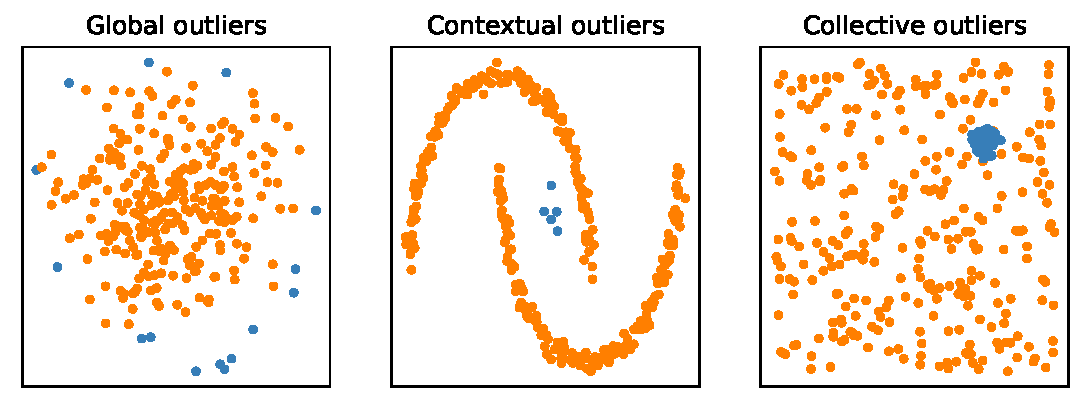
\includegraphics[width=0.7\textwidth]{../imgs/outlier_examples.pdf}
        \caption{Types of outliers}
    \end{figure}

    \begin{itemize}
        \item \textbf{Fig 1a:} Global outliers
        \item \textbf{Fig 1b:} Contextual outliers -- Given the dataset has two clusters, each one has a moon shape.
        \item \textbf{Fig 1c:} Blue points are collective outliers because the density of those points is much higher than the rest.
    \end{itemize}

\end{frame}

%-------------------------------------------------------------------------------
\begin{frame}
    \frametitle{2020 361 Exam Question 4 -- Outlier / Anomaly Detection}
    \small

    The following figure shows the monthly telecom usage activity in a specific area across
    several years. You were tasked to identify whether outliers exist in the data.

    \begin{figure}
        \centering
        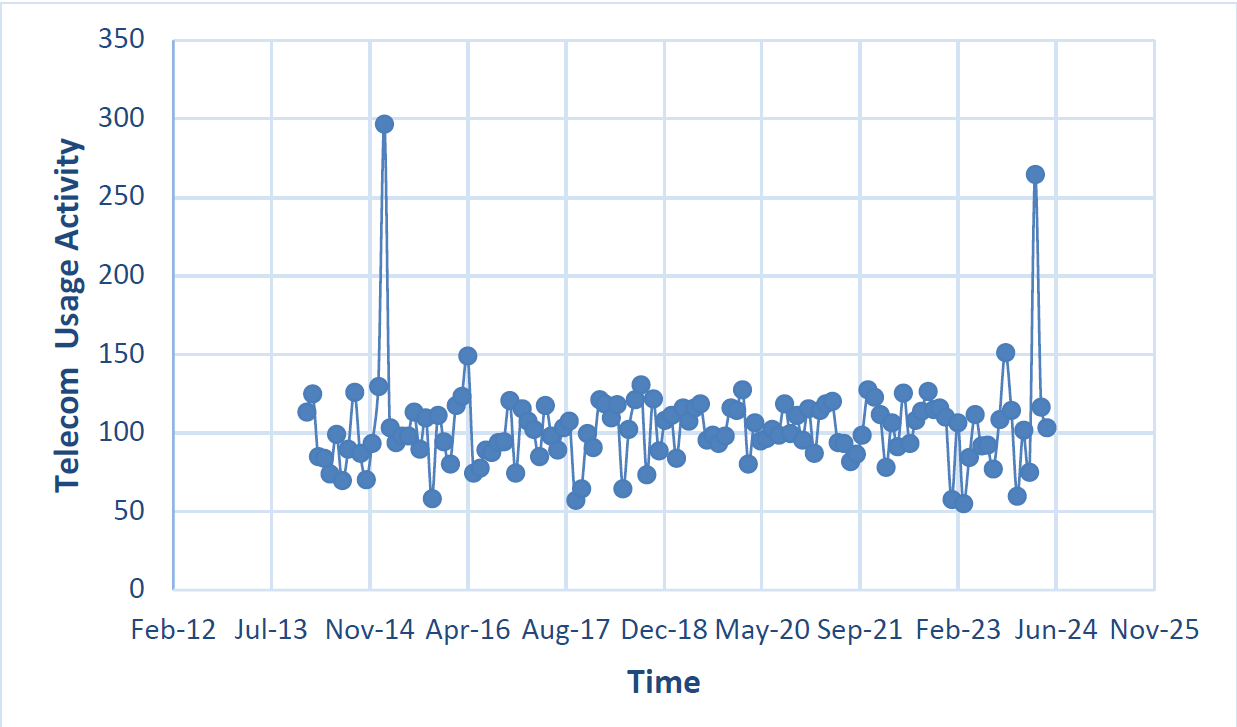
\includegraphics[width=0.6\textwidth]{../imgs/question4.png}
        % \caption{Monthly telecom usage}
    \end{figure}
    
    What outlier detection technique would you use to identify whether outliers exist for this case?
\end{frame}

%-------------------------------------------------------------------------------
\begin{frame}
    \frametitle{2020 361 Exam Question 4 -- Outlier / Anomaly Detection}

    \begin{columns}[]
        \begin{column}{0.5\textwidth}
            \begin{figure}
                \centering
                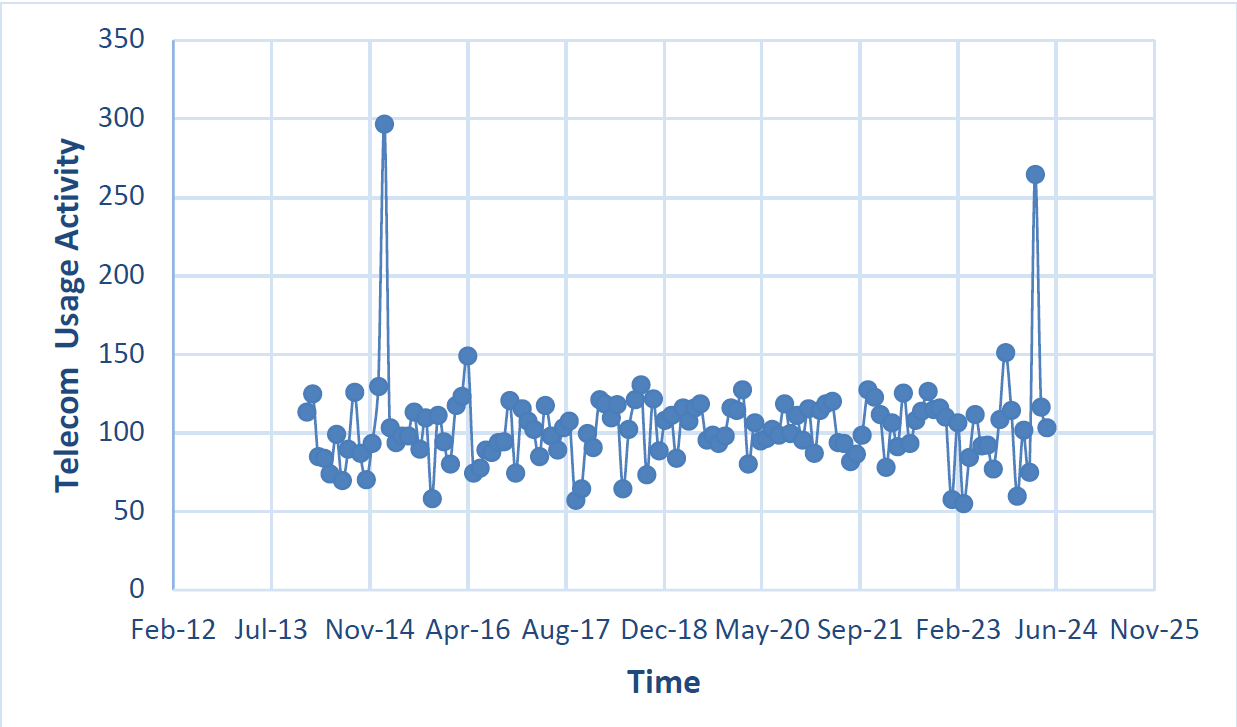
\includegraphics[width=\textwidth]{../imgs/question4.png}
                % \caption{Monthly telecom usage}
            \end{figure}
        \end{column}
        \begin{column}{0.5\textwidth}
            \begin{itemize}
                \item No obvious periodic pattern;
                \item No dramatic density changes;
                \item Unlikely to have contextual outlier and collective outlier;
                \item We apply the \textbf{statistical approach -- parametric method} to find global outliers.
                \item There are multiple ways to solve this problem.
            \end{itemize}
        \end{column}
    \end{columns}
    
\end{frame}

%-------------------------------------------------------------------------------
\begin{frame}
    \frametitle{2020 361 Exam Question 4 -- Outlier / Anomaly Detection}
    
    \begin{columns}[]
        \begin{column}{0.5\textwidth}
            \begin{figure}
                \centering
                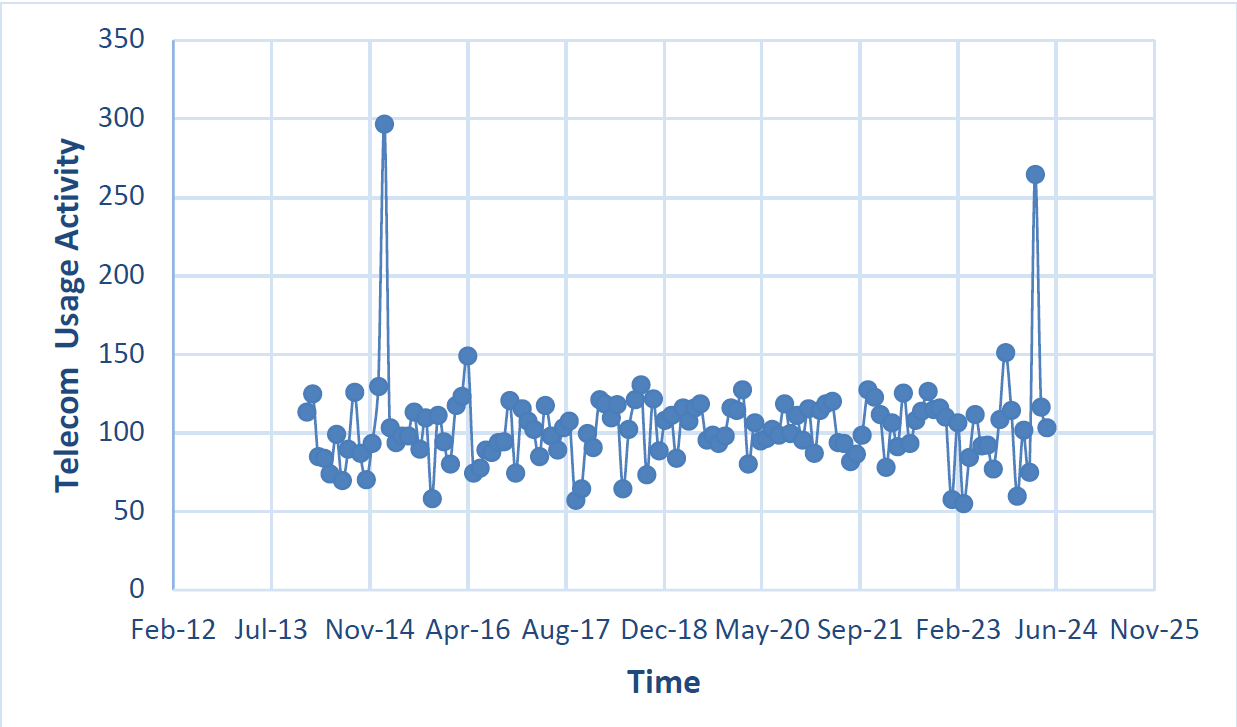
\includegraphics[width=\textwidth]{../imgs/question4.png}
                % \caption{Monthly telecom usage}
            \end{figure}
        \end{column}
        \begin{column}{0.5\textwidth}
            \begin{itemize}
                \item \textbf{Parametric method:} Assume the samples are drawn from a normal distribution, estimate the maximum likelihood of mean $\mu$ and standard deviation $\sigma$.
                \item We know that the $\mu \pm 3 \sigma$ region contains $99.7\%$. According to z-score, if $z=\frac{|x_i-\bar{x}|}{s} > 3$, the sample $x_i$ is generated by the normal distribution is less than $\frac{0.3}{2}=0.15\%$.
                \item Note that we do not know the population mean and standard deviation, we only have sample mean and sample standard deviation.
            \end{itemize}
        \end{column}
    \end{columns}

\end{frame}

%-------------------------------------------------------------------------------
\begin{frame}
    \frametitle{2020 361 Exam Question 4 -- Outlier / Anomaly Detection}
    
    \begin{columns}[]
        \begin{column}{0.5\textwidth}
            \begin{figure}
                \centering
                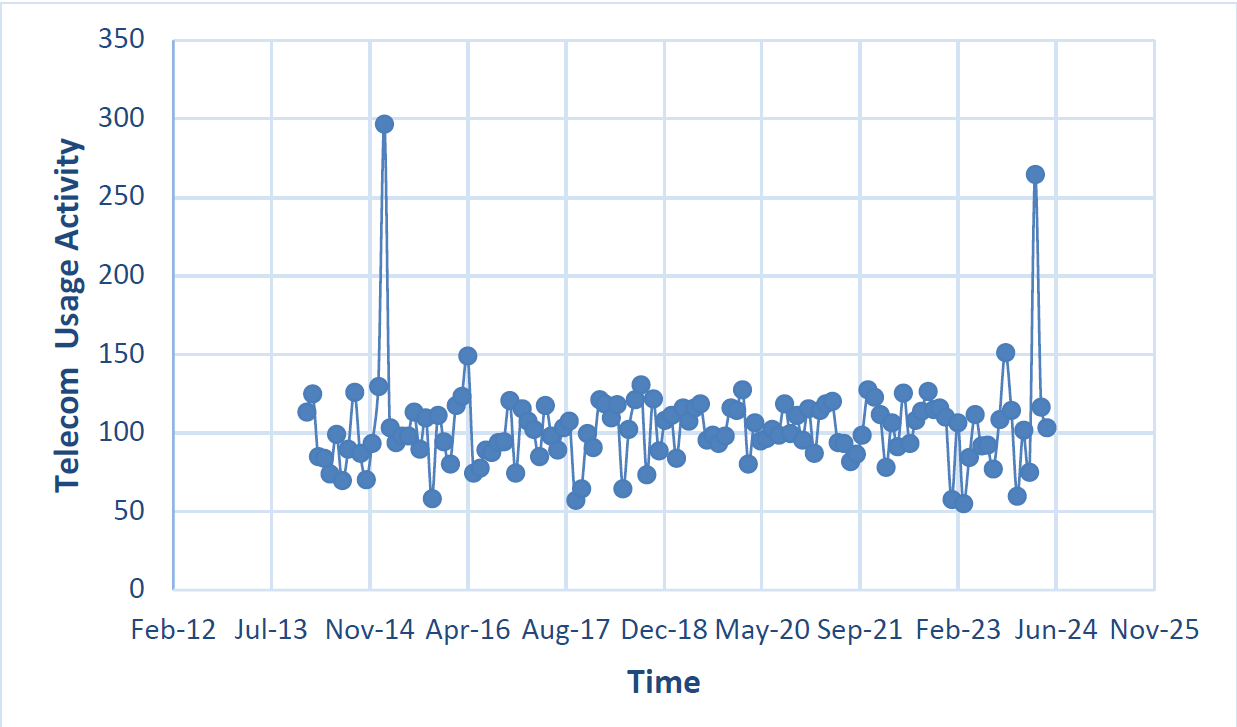
\includegraphics[width=\textwidth]{../imgs/question4.png}
                % \caption{Monthly telecom usage}
            \end{figure}
        \end{column}
        \begin{column}{0.5\textwidth}
            \begin{itemize}
                \item Based on observation, each grid contains around 14 points, we have 110 data points in total. 
                \item $\bar{x} = \frac{1}{N}\sum^N_{i=1}x_i \approx 100$
                \item $s = \sqrt{\frac{1}{N-1}\sum^N_{i=1}(x_i - \bar{x})^2} \approx 20$
                \item $\frac{|300 - 100|}{20}=10 > 3$, an outlier
                \item $\frac{|270 - 100|}{20}=8.5 > 3$, an outlier
                \item $\frac{|150 - 100|}{20}=2.5 < 3$, not an outlier
                \item $\frac{|55 - 100|}{20}=2.25 < 3$, not an outlier
            \end{itemize}
        \end{column}
    \end{columns}

\end{frame}

%-------------------------------------------------------------------------------
\begin{frame}
    \frametitle{Tutorial Question 1 -- Anomaly Detection}
    
    \begin{block}{Question 1}
        You are given the following list of 2D data points. 
        [[1; 1]; [1; 2]; [2; 2]; [2; 1]; [3; 3]; [2; 5]; [2; 3]] If you had to select one point to be anomalous, 
        which would you pick? Explain your answer. Please link your explanation to an anomaly detection technique.
    \end{block}



    There are multiple ways to solve this problem.\\
    Let's use \textbf{distance-based outlier detection}.


\end{frame}

%-------------------------------------------------------------------------------
\begin{frame}[t]
    \frametitle{Tutorial Question 1 -- Anomaly Detection}
    \small
    
    \begin{columns}[t]
        \begin{column}{0.5\textwidth}
            \textbf{Distance-based outlier detection}

            \begin{table}[]
                \scriptsize
                \begin{tabular}{c|ccccccc}
                             & \textbf{1,1} & \textbf{1,2} & \textbf{2,2} & \textbf{2,1} & \textbf{3,3} & \textbf{2,5} & \textbf{2,3} \\ \hline
                \textbf{1,1} & 0            & 1            & 2            & 1            & 4            & 5            & 3            \\
                \textbf{1,2} & 1            & 0            & 1            & 2            & 3            & 4            & 2            \\
                \textbf{2,2} & 2            & 1            & 0            & 1            & 2            & 3            & 1            \\
                \textbf{2,1} & 1            & 2            & 1            & 0            & 3            & 4            & 2            \\
                \textbf{3,3} & 4            & 3            & 2            & 3            & 0            & 3            & 1            \\
                \textbf{2,5} & 5            & 4            & 3            & 4            & 3            & 0            & 2            \\
                \textbf{2,3} & 3            & 2            & 1            & 2            & 1            & 2            & 0           
                \end{tabular}
                \caption{Manhattan Distance Matrix}
            \end{table}

            \[
                \frac{\norm{\{o' | \text{dist}(o, o') \le r\}}}{\norm{D}} \le \pi
            \]

            We need to define the hyperparameters: $r$ and $\pi$.
        \end{column}
        \begin{column}{0.5\textwidth}
            The number of data points, $\norm{D}$, is 7.\\
            Let $r=2$,

            \begin{table}[]
                \scriptsize
                \begin{tabular}{c|c|c}
                             &  \textbf{\# of objects within $r$} & \textbf{Divide by $\norm{D}$}\\ \hline
                \textbf{1,1} &  3 & 0.43 \\
                \textbf{1,2} &  4 & 0.57 \\
                \textbf{2,2} &  5 & 0.71 \\
                \textbf{2,1} &  4 & 0.57 \\
                \textbf{3,3} &  2 & 0.29 \\
                \rowcolor[HTML]{34CDF9}\textbf{2,5} &  1 & 0.14 \\
                \textbf{2,3} &  5 & 0.71   
                \end{tabular}
                \caption{The \# of neighbours within $r$}
            \end{table}

            If we select only one point as an outlier, we can set $\pi$ to any value between $0.14$ and $0.29$, e.g. $0.15$.\\
            Therefore, we identify $[2;5]$ is an outlier.\\            
        \end{column}
    \end{columns}
\end{frame}


%-------------------------------------------------------------------------------
\begin{frame}
    \frametitle{}
    
    
\end{frame}

%-------------------------------------------------------------------------------
\begin{frame}
    \frametitle{}
    
    
\end{frame}

%-------------------------------------------------------------------------------
\begin{frame}
    \frametitle{}
    
    
\end{frame}

%-------------------------------------------------------------------------------
\begin{frame}
    \frametitle{}
    
    
\end{frame}

%-------------------------------------------------------------------------------
\begin{frame}
    \frametitle{}
    
    
\end{frame}

%-------------------------------------------------------------------------------
\begin{frame}
    \frametitle{}
    
    
\end{frame}

%-------------------------------------------------------------------------------
\begin{frame}
    \frametitle{}
    
    
\end{frame}


\end{document}


